\chapter{CNN Background}
\label{chapter:background}

%This chapter is the main one for the IIEEC report, it contains the section about \textbf{Framing of the thesis theme in the scientific area and state of the art revision}.
%%%%%%%%%%%%%%%%%%%%%%%%%%%%%%%%%%%%%%%%%%%%%%%%%%%%%%%%%%%%%%%%%%%%%%%%%
%
%Things I need to talk about:
%\begin{itemize}
%    \item What are neural networks being used for - general introduction
%    \item architecture of neural networks: more terminology: input, output, hidden layers...
%    \item Training vs Inference
%    \item Basic neural network operations: weights, biases, Activations (Fully Connected Layer)
%    \item Deep neural networks: advantages, difficulties
%    \item Convolutional Neural Networks (CNN): basic operation, some intuition, results (e.g ImageNet)
%    \item 3 basic ideias of CNNs: local receptive fields, shared weights, pooling
%    \item introduce terminology: kernel/filter, feature map
%    \item putting all factors that make DNNs, more specifically CNNs work
%    \item factors for effective training (and problems)
%\end{itemize}{}
%
%\newpage

Convolutional neural networks (CNNs) were introduced in 1989 by Yann LeCun for
digit recognition~\cite{lecun:handwritten_zipcodes89}. Since then CNNs have
increased in size and complexity and have gained popularity in the last years
for applications like speech processing, robotics and image processing. One
example is the performance of AlexNet~\cite{AlexNetKrizhevsky:2012} at the
ImageNet Large Scale Visual Recognition Challenge
2012~\cite{ImageNet2012_ILSVRC15}.

In this chapter a background for CNNs is established. The first sections
introduce the concepts of inference and training of neural networks. Then, the
main types of layers found in CNNs are presented. In the final part of the
chapter, an analysis of the YOLOv3~\cite{yolov3} network, a CNN used for image
detection, is presented.


%Since the result of the AlexNet \cite{AlexNetKrizhevsky:2012} at the ImageNet Large Scale Visual Recognition Challenge 2012 \cite{ImageNet2012_ILSVRC15}, convolutional neural networks have been used for image recognition applications.

\section{Neural Networks}
\label{section:neural_networks}

% Neural networks have gained popularity in the last years due to accuracy on applications like speech processing, robotics and image processing.
\begin{figure}[!htb]
	\centering
	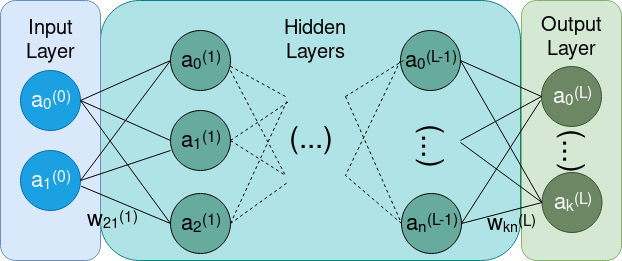
\includegraphics[width=0.70\textwidth]{Figures/FCNN.png}
	\caption[Caption for figure in TOC.]{Neural Network Structure}
	\label{fig:FCNN}
\end{figure}

The most basic element of neural networks is the neuron. The output value $a$ of
a neuron is given by
\begin{equation}
a  = \sigma\Big( b + \sum_{i=0}^{n-1} w_{i}\times x_i \Big),
\label{eq:neuron_value}
\end{equation}
where $w_i$ is the weight associated with input $x_i$, $b$ is a parameter called
bias, $\sigma(.)$ is called the activation function and $n$ is the number of
inputs of the neuron.

Fig.~\ref{fig:FCNN} presents a neural network. Neurons are organized in layers
where the neurons in one layer only receive input values from the same set of
previous layers. If the input values are the neural network inputs, the layer is
called the \underline{input layer}. The values calculated at the input layer
neurons are sent to the next layer. The last layer of the network is called the
\underline{output layer}. The layers in between are called \underline{hidden
  layers}.

Activations are non-linear functions applied to each neuron output. The non-linearity
of the activation functions allows for multiple layer networks to approximate
any function~\cite{mnielsen:nnanddl}. The sigmoid function, presented in
Fig.~\ref{fig:sigmoid}, is one of the first functions used. In the last years,
the Rectified Linear Unit (ReLU), Fig.~\ref{fig:ReLU}, and some variations like
the leaky ReLU, Fig.~\ref{fig:leaky}, have gained popularity due to the reduced
computational complexity during network training.
%\begin{equation}
%\begin{cases}
%Sigmoid(x) = \frac{1}{1 + \exp(-x)} \\
%ReLU(x) = max\{0, x \}\\
%Leaky_{ReLU}(x) = max\{0.1x, x\}
%\label{eq:activation_functions}
%\end{cases}
%\end{equation}

\begin{figure}[!htb]
	\begin{subfigmatrix}{3}
		\subfigure[Sigmoid Activation]{\label{fig:sigmoid} 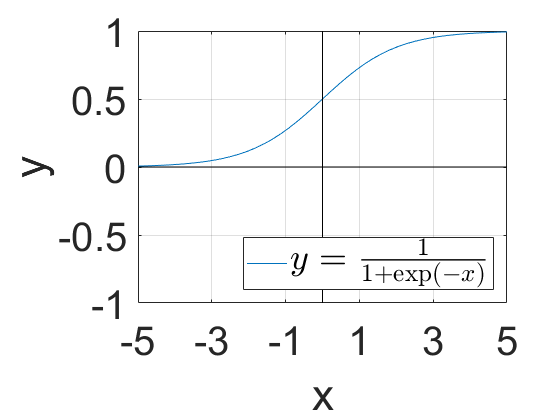
\includegraphics[width=0.32\textwidth]{Figures/sigmoid.png}}
		\subfigure[ReLU Activation]{\label{fig:ReLU} 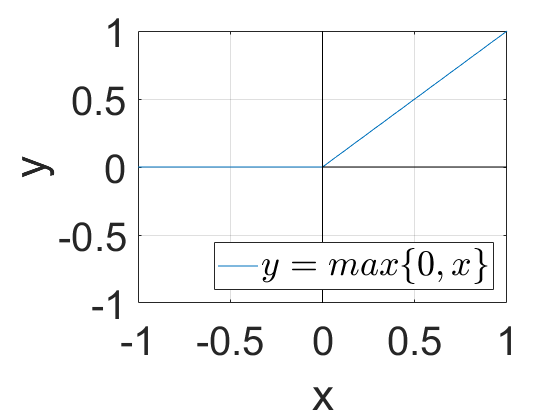
\includegraphics[width=0.32\textwidth]{Figures/ReLU.png}}
		\subfigure[Leaky ReLU Activation]{\label{fig:leaky} 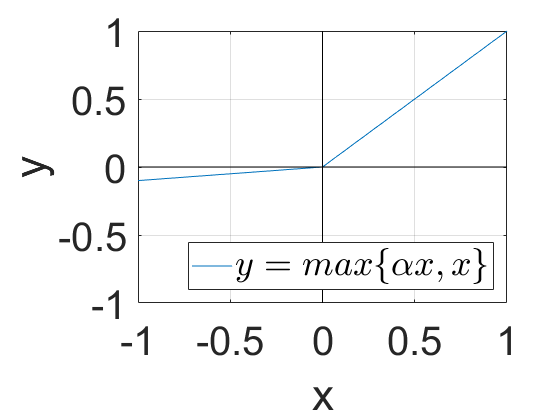
\includegraphics[width=0.32\textwidth]{Figures/leaky_ReLU.png}}		
	\end{subfigmatrix}
	\caption{Plots of common activation functions}
	\label{fig:activation_plots}
\end{figure}

\section{Neural Network Inference}
\label{section:inference}
Inference corresponds to the operation of the network over data outside of the
training dataset using the already trained weights and biases. The key idea
behind this mode is that if the input data being received is similar to the data
used for training, then the output generated by the network should reach a
comparable accuracy with the one achieved during training.

\section{Neural Network Training}
\label{section:training}
Neural networks are trained using a training dataset that contains inputs for
the network and the desired outputs. During training, the weights and biases of
the network are tuned so that given the dataset inputs, the output generated is
as close as possible to the desired output. Training is based on gradient
descent techniques that update the weights and biases of the network based on
the partial derivatives of each value with respect to the difference between the
desired output and the one generated by the network. The backpropagation
algorithm is the main method used for network training. Training is demanding in
terms of computation and memory. The training process is often done in a
separate machine, usually taking advantage of the computation capabilities of
GPUs.

\section{Fully-Connected Network}
\label{subsection:fc_network}

In fully-connected layers, each neuron receives the outputs from all neurons of
the previous layer, where there is a different weight associated for each input
value. In fact, Fig.~\ref{fig:FCNN} depicts a neural network composed
exclusively by fully-connected layers.


%In general the fully-connected layers appear at the end of the network to perform the classification of the features detected by the convolutional layers.

%intro to deep neural networks into CNNs
% 3 basic ideias - introduce terminology
% talk about convolution - pooling - normalization - activations
% quantitative factors to CNNs (throughout the previous text?)

%\subsection{Deep Neural Networks (DNNs)}
%\label{subsection:dnns}
%For the application of image processing, the intuition of how the network works is related with each neuron being able to detect one pattern. With more layers, the neurons on the first layers detect simple patterns that are progressively compounded into more complex patterns across the layers, up to the output layer, where the object detection is done. Following this logic, it is expected that deep neural networks can be more powerful than a shallow network. However, this comes with additional difficulties in training all the weights and biases for networks of increasing depth. This problem is usually circumvented by replacing the fullyconnected layers with convolutional layers.

\section{Convolutional Neural Networks (CNNs)}
\label{section:cnns}

Unlike fully-connected networks, CNNs are mainly composed by convolutional
layers. Other commonly found layers in CNNs are pooling, batch normalization,
routing, upsample and shortcut layers.

% Convolutional neural networks are based on three basic ideas: \underline{local receptive fields}, \underline{shared weights} and \underline{pooling} \cite{mnielsen:nnanddl}.


\subsection{Convolutional Layer}
\label{subsection:conv_layer}

In convolutional layers, a neuron only depends on a small number of inputs,
which corresponds to the neuron only analysing a specific feature for a region
of the input. The specific region is called local receptive
  field. Hence, associated with each neuron, there is only a reduced number of
weights and one bias.

In fact, the same local weights and bias are used for a set of neurons, which
corresponds to searching for the same feature in the entire input, making
convolution invariable to translation in images. The shared weights form a
\underline{kernel}.

%This process creates a \underline{feature map (FM)} of the input, due to using the same \underline{shared weights} and \underline{shared bias} over a small region that is overlapped onto an image like a sliding window. 
% and for each layer multiple kernels can be used to generate multiple corresponding feature maps.

The input of convolutional layers is divided into $C$ channels, where each
channel is defined as a ($W\times H$) \underline{feature map (FM)}. For example,
in Fig.~\ref{fig:3D_conv} the input has 3 channels and each feature map has size
$6\times 6$.

Each kernel used in the convolution has $C$ channels, the same as the input. The
number of output channels is the same as the number of kernels used. Each value
on the output is the accumulation of the products of the input with the
overlapped kernel.

\begin{figure}[!htb]
	\centering
	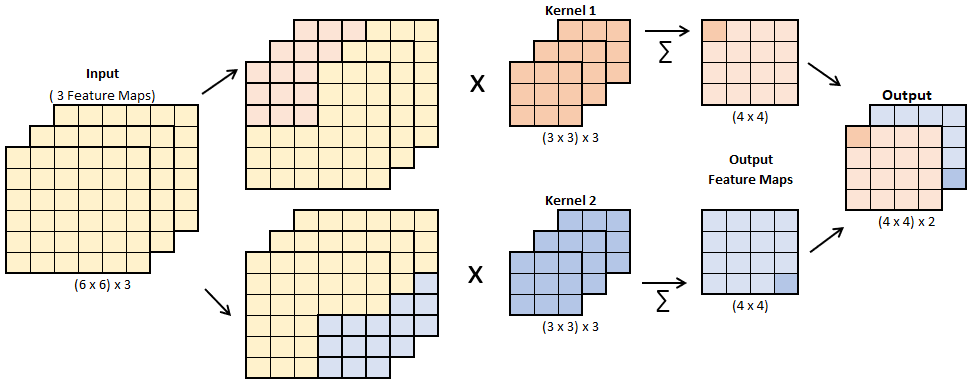
\includegraphics[width=0.70\textwidth]{Figures/3D_convolution.png}
	\caption[Caption for figure in TOC.]{Example of a 3D convolution}
	\label{fig:3D_conv}
\end{figure}

%Fig. \ref{fig:3D_conv} presents an example of a 3D convolution. Given an input composed of multiple feature maps (channels), multiple three dimensional kernels with the same number of channels are used for convolution, creating one output feature map per kernel. The number of output channels is the same as the number of kernels used. Each value on the output is the accumulation of the products of the input with the overlapped kernel.

\subsection{Pooling Layer}
\label{subsection:pool_layer}
CNNs commonly use \underline{pooling} layers to reduce the size of the feature
maps. Intuitively this corresponds to only keeping a rough idea of the feature
location. The reduction of the feature maps also reduces the amount of
computation at latter layers of the network. The most common pooling operations
divide the feature map into $2\times2$ regions and select either the larger
(Max-pooling) or the average (Average-pooling) value.

% figure of max pooling?

\subsection{Batch Normalization Layer}
\label{subsection:batch_norm_layer}
Batch normalization sets the average of the input values to zero and the
standard variation to one. After that, the values are scaled and shifted using
the ($\gamma$,$\beta$) parameters also learned in training. This control of the
input distribution speeds up training and improves
accuracy~\cite{sze:dnn_tutorial}. For a given value $x$, the normalization
outputs

%As the depth of the network increases, the input value distribution across
%layers is a factor that can impact the speed of training. That problem is
%reduced with batch normalization that sets the average to zero and the standard
%variation to one and then the value is scaled and shifted using the
%($\gamma$,$\beta$) parameters also learned in training. For a given value $x$,
%the normalization outputs

\begin{equation}
y = \frac{x - \mu}{\sqrt{\sigma^2 + \epsilon}}\gamma + \beta
\label{eq:batch_normalization}
\end{equation}
Since all variables are known after training, is possible to rewrite (\ref{eq:batch_normalization}) as 
\begin{equation}
\frac{\gamma}{\sqrt{\sigma^2 + \epsilon}}x + \Bigg(-\frac{\mu}{\sqrt{\sigma^2 + \epsilon}}\gamma + \beta  \Bigg) = Ax + B,
\label{eq:batch_normalization_macc}
\end{equation}
which avoids the computation of the square root and division.  The additional
$\epsilon$ term is used to avoid numerical errors related with denominators too
close to zero.

\subsection{Routing Layer}
\label{subsection:route_layer}
Routing layers are used to get an output from a previous layer in the network. If multiple previous layers are selected, their output is concatenated.

\subsection{Upsample Layer}
\label{subsection:upsample_layer}
Upsample layers increase the size of the input FMs, doubling their width and
height. The simplest upsample method consists in repeating each value in a FM
four times in a $2\times 2$ square.

\subsection{Shortcut Layer}
\label{subsection:shortcut_layer}
Shortcut layers add the output from two or more previous layers in the network
pipeline. Shortcut layers are used to mitigate the vanishing gradient problem
that arises during training for networks with considerable depth. With this
addition, the networks act as already knowing the result from the further back
layer and only need to learn a residual to get the desired outcome. Shortcut
layers are common on ResNet
networks~\cite{ResNet_2015DBLP:journals/corr/HeZRS15}.

\section{YOLO}
YOLO (You Only Look
Once)~\cite{Yolov1_DBLP:journals/corr/RedmonDGF15,Yolov2_redmon2016yolo9000,yolov3}
is an object detection and classification system that is composed of a single
CNN that receives an image and outputs bounding box coordinates and class
probabilities from the detected objects.

A YOLO network is composed of a sequence of convolutional layers that serve as
feature extractors at different scales. During these layers of the network, the
size of the FMs is gradually reduced whether by pooling layers or convolutional
layers with stride 2, depending on the network version.

After the feature extraction, object detection and classification is done at
different FM sizes, which corresponds to analysing the input image at different
$g_i \times g_i$ grids.

For each cell in each grid, $M$ attempts of object detection are done. Each
attempt is represented by \underline{two} values for the \underline{object box
  center}, \underline{two} for the \underline{object box size}, \underline{one}
value for the \underline{objectness score} and \underline{80 class scores}. The
objectness score indicates the likelihood of the detection corresponding to an
object. The 80 class scores correspond to the number of existing classes in the
COCO dataset~\cite{coco:Microsoft} used for training. In total an object
detection attempt is represented by $(2+2+1+80) = 85$ values.

Before the object detection and classification at grid size $g_i \times g_i$
starts, a set of $(M \times 85)$ FMs of size $ g_i \times g_i$ is created, and
each detection value is associated with a specific FM.

%In total there are $ M \times (1+2+2+80) = M\times 85$ values per grid cell,
%which corresponds to the $M\times 85$ FMs at the input of the yolo layers. The
%size of each FM at the yolo layer input corresponds to the grid size used for
%the detection.


%Each attempt is represented by one value for the objectness score, which
%indicates the likelihood of the detection corresponding to an object; two
%values for the object box position and two for the object box size; and 80
%scores, one for each class being classified. In total there are $ 3 \times
%(1+2+2+80) = 255$ values per grid cell, which corresponds to the $255$ FMs at
%the input of the yolo layers. The size of each FM at the yolo layer input
%corresponds to the grid size.

The object detection and classification process uses a custom type of layer
called \underline{yolo layer}. At the yolo layers, the FMs of the channels
corresponding to the \underline{box coordinates}, \underline{objectness score}
and \underline{classes scores} are passed through a sigmoid activation function
(Fig.~\ref{fig:sigmoid}). The channels for each output type and the activation
performed at the yolo layer is presented in
Tab.~\ref{tab:yolov3_channel_division}, for the case of $M=3$. The outputs of
the several yolo layers correspond to the outputs of the network.

\begin{table}[!htb]
	\renewcommand{\arraystretch}{1.2} % more space between rows
	\centering
	\begin{tabular}{ccc}
		\toprule
		Channel Ranges           & Outputs & Activation  \\
		\midrule
		$\{[0,1];[85,86];[170,171]\}$       & Box center coordinates   & Sigmoid \\
		$\{[2,3];[87,88];[172,173]\}$       & Box size   & None \\
		$\{4;89;174\}$       & Objectness score   & Sigmoid \\
		$\{[5-84];[90-169];[175-254]\}$       & Class scores   & Sigmoid \\
		\bottomrule
	\end{tabular}
	\caption[Table caption shown in TOC.]{Yolo layer channel composition and performed activations for $M=3$.}
	\label{tab:yolov3_channel_division}
\end{table}

After all the outputs of the network are obtained, all the detections done by
the network need to be filtered. This consists in excluding detections with an
objectness score below a determined threshold; and then applying Non-maximum
Suppression (NMS) to eliminate multiple detections of the same object. The NMS
process starts from the detection with highest objectness score and resorts to a
Intersection over Union (IoU), illustrated in Fig.~\ref{fig:IoU}, 
between the current detection box and all the
others. If the result is above the IoU
threshold, the detection with the lowest objectness score is discarded,
otherwise it is kept. This is done for all remaining detections in a descending
order of objectness score.
\begin{figure}[!htb]
	\centering
	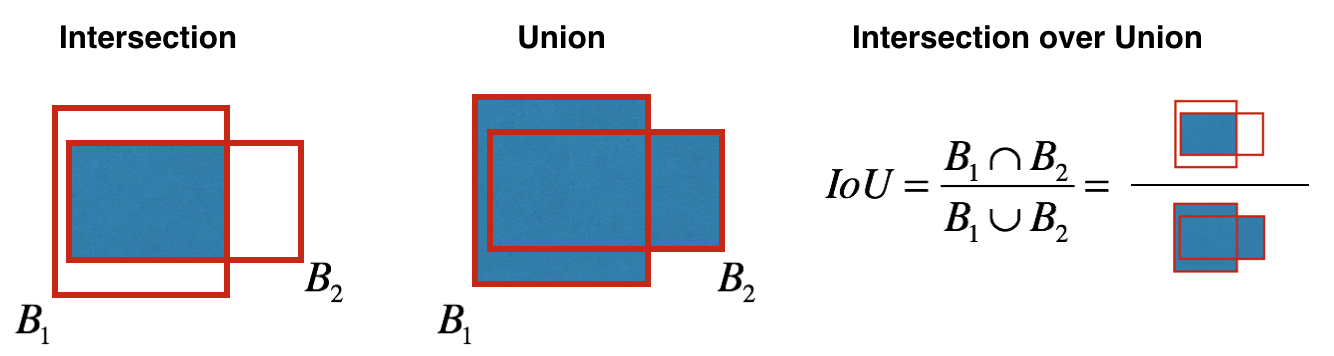
\includegraphics[width=0.5\textwidth]{Figures/IoU.png}
	\caption[Caption for figure in TOC.]{Diagram of the Intersection over Union (IoU) calculation, from~\cite{IoU_image_credit}}
	\label{fig:IoU}
\end{figure}

\subsection{Accuracy Metrics}
\label{sec:map}


The mean Average Precision (mAP) is a measure used to compare networks that use the Common Objects in
Context (COCO) dataset~\cite{coco:Microsoft}.

%FIX explanation
%The mAP metric gives an indication of the degree to which the correct
%classification have the highest confidence levels.
%???(FIXED) - isto não esta aqui a fazer nada, mas vale nao confundir


The mAP is the average of the
AP calculated for each class. The AP is calculated by ordering the
classifications performed by the highest bounding box confidence level. The
classifications are evaluated as true positives or false positives according to the ground truth. At each classification is also calculated the precision and recall, given by
\begin{equation}
	recall = \frac{\#True \ Positives}{\# Total True Positives} \text{ and } precision = \frac{\# True \ Positives}{\# Classifications}.
	\label{eq:precision_recall}
\end{equation}
The true positives are the number of correct classifications up to the classification being analysed and the total true positives are the total number of objects in the image. The number of classifications corresponds to the order of the classification being analysed. A precision/recall curve is calculated with the values computed for each classification as is presented by the orange curve in Fig.~\ref{fig:mAP}. The curve is then altered in order to have monotonically decreasing precision, by setting the precision at a given point equal to the maximum precision for any value of higher recall, as is presented by the green curve in Fig.~\ref{fig:mAP}. Finally, the AP is calculated by computing the area under the green curve.
%The mAP is the average of the
%AP calculated for each class. The AP is calculated by ordering the
%classifications performed by the highest bounding box confidence level. The
%classifications are evaluated as true positives or false positives according to the ground truth. From each
%true positive found onwards, the classifications receive the score of the recall
%at the true positive.
% how to decide if true or false?
\begin{figure}[!htb]
	\centering
	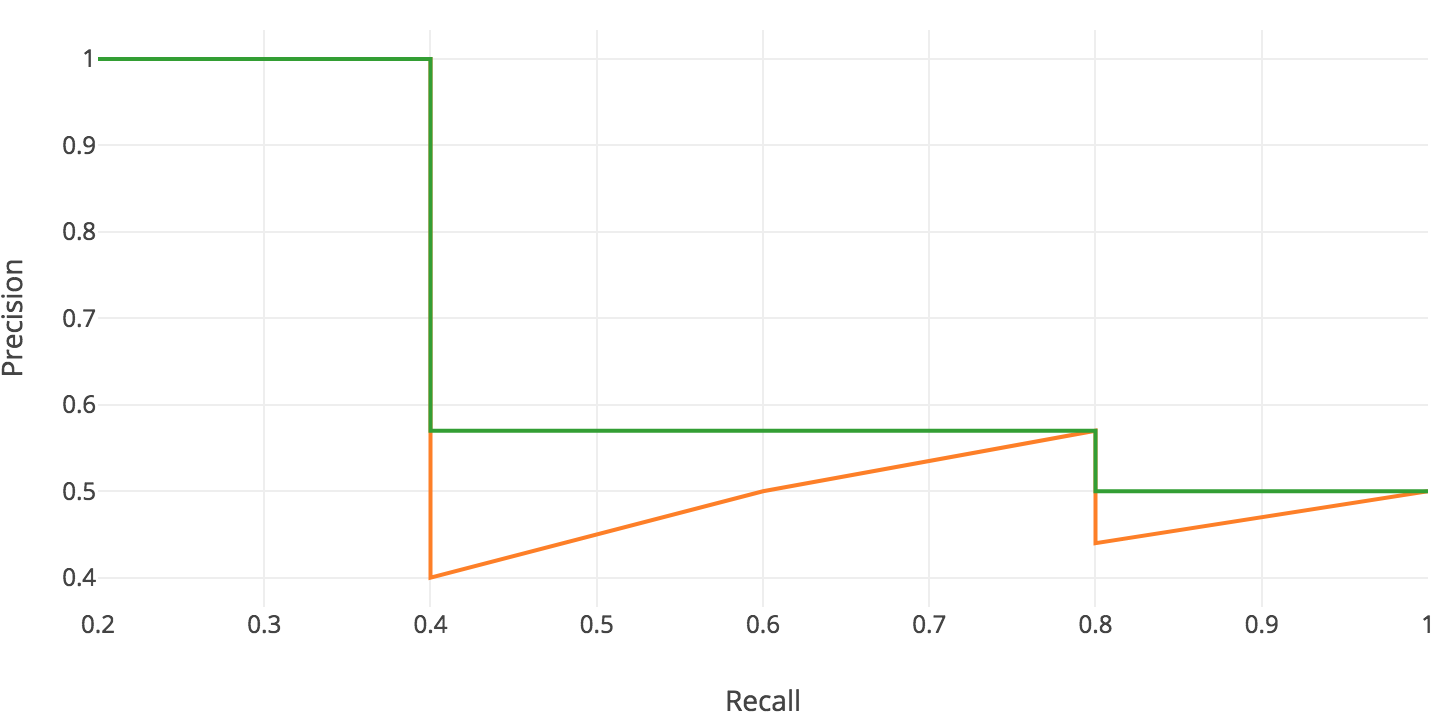
\includegraphics[width=0.5\textwidth]{Figures/mAP.png}
	\caption[Caption for figure in TOC.]{Example of precision/recall curve, adapted from~\cite{mAP}}
	\label{fig:mAP}
\end{figure}

%The score of classification $k$ is defined as interpolated
%precision ($P_{inter}(k)$).
%
%%how to compute Pinter ?
%
%
%With the number of ground truth positives (GTP), the
%AP is calculated by
%
%%what is GTP?
%
%\begin{equation}
%AP = \frac{1}{GTP} \sum_{i = 0}^{N} P_{inter}(i),
%\label{eq:AP}
%\end{equation}
%%END FIX (FIXED) - acabei por adicionar uma imagem, para mim é 1000x melhor do que qualquer texto que eu escreva
%where N is the total number of classifications above the IoU level.

Tab.~\ref{tab:yolov3_performance_metrics} presents the mAP
for a 0.5 IoU threshold and respective inference time (in ms) for
multiple networks. The results were obtained using machines with an M40 or Titan
X Pascal GPUs~\cite{yolov3} as indicated. The results show that the
Yolov3 networks achieve an accuracy on pair with the best performing networks at
a fraction of their inference time. The different versions of the Yolov3
networks are related with the resolution of the input images, but all have the
network structure.

\begin{table}[!htb]
	\renewcommand{\arraystretch}{1.2} % more space between rows
	\centering
	\begin{tabular}{lcccc}
		\toprule
		Network           & $mAP_{50}$ & Time (ms) & FPS & GPU  \\
		\midrule
		SSD321		& 45.4	& 61 & 16.4 & M40\\
		DSDSD321	& 46.1	& 85 & 11.8& M40\\
		R-FCN		& 51.9	& 85 & 11.8& M40\\
		SSD513		& 50.4	& 125 & 8& M40\\
		DSSD513		& 53.3	& 156 & 6.4& M40\\
		FPN FRCN	& \textbf{59.1} & 172 & 5.8& M40\\
		RetinaNet-50-500 & 50.9	& 73 & 13.7& M40\\
		RetinaNet-101-500 & 53.1	& 90 & 11.1& M40\\
		RetinaNet-101-800 & 57.5	& 198 & 5.1& M40\\
		Yolov3-320 & 51.5	& \textbf{22} & \textbf{45.5}& Titan X Pascal\\
		Yolov3-416 & 55.3	& 29 & 34.5& Titan X Pascal\\
		Yolov3-608 & 57.9	& 51 & 19.6& Titan X Pascal\\
		\bottomrule
	\end{tabular}
	\caption[Table caption shown in TOC.]{mAP and inference time comparison between multiple networks, adapted from~\cite{yolov3, Focal_Loss}.}
	\label{tab:yolov3_performance_metrics}
\end{table}

\subsection{Yolov3}
\label{sec:yolov3}
As presented in Tab.~\ref{tab:yolov3_performance_metrics}, the Yolov3 network
performs object detection at a higher framerate than other networks, while
maintaining a comparable level of accuracy.

\begin{table}[!htb]
	\renewcommand{\arraystretch}{1.2} % more space between rows
	\centering
	\begin{tabular}{lc}
		\toprule
		Layer Type           & Number of Layers  \\
		\midrule
		Convolutional       & 75    \\
		Shortcut  			& 23     \\
		Route 			    & 4     \\
		Yolo  				& 3     \\
		Upsample 		    & 2     \\
		Total 				& 107 \\
		\bottomrule
	\end{tabular}
	\caption[Table caption shown in TOC.]{Yolov3 layer type composition.}
	\label{tab:yolov3_num_layers}
\end{table}
Tab.~\ref{tab:yolov3_num_layers} presents the layer composition of the Yolov3
network. The majority of the layers are convolutional. Most of the convolutional
layers are used for feature detection or for reducing the FM resolution. This network
uses convolutional layers with $3\times3$ kernels with stride 2 instead of
pooling layers.

Due to the depth of the network, shortcut layers are used, to tackle the
problems described in section ~\ref{subsection:shortcut_layer}.

The accuracy performance for small object detection also comes from using three
different cell grid scales as opposed to the two used in previous
versions~\cite{Yolov2_redmon2016yolo9000}: ($13\times13$), ($26\times26$) and
($52\times52$). The indicated resolutions are specific to the Yolov3-416
version.

Fig.~\ref{fig:yolov3_stages} presents the main stages that constitute recurring
sequences of layers in the network: the F stage presented in
Fig.~\ref{fig:F_Stage} and the Yolo stage presented in
Fig.~\ref{fig:Yolo_Stage}.

\begin{figure}[!htb]
	\begin{subfigmatrix}{2}
		\subfigure[F stage composition]{\label{fig:F_Stage} 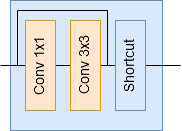
\includegraphics[width=0.25\textwidth]{Figures/FStage.png}}
		\subfigure[Yolo stage composition]{\label{fig:Yolo_Stage} 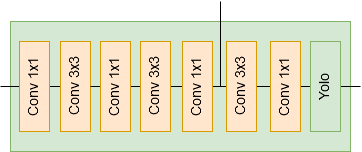
\includegraphics[width=0.50\textwidth]{Figures/YoloStage.png}}	
	\end{subfigmatrix}
	\caption{Stages of Yolov3 Network}
	\label{fig:yolov3_stages}
\end{figure}

Each F stage is composed of a convolutional layer with $1\times1$ kernels followed by
another with $3\times3$  kernels. At the end of the stage there is a shortcut layer
that adds the outputs of the second layer to the input of the stage.

In each Yolo stage, there is a sequence of convolutional layers, with $3\times
3$ and $1\times 1$ kernels that generate FMs of size $13 \times 13$ into the
first yolo layer. Since Yolov3 performs three detection attempts per grid cell,
there are $3\times 85 = 255$ FMs as input for every yolo layer. The
classification takes place for a grid with the same size as the FMs and the
number of FMs corresponds to the number os parameters to be calculated per grid
cell.

A complete scheme of the network is presented in Fig.~\ref{fig:Yolov3_complete}.

\begin{figure}[!htb]
	\centering
	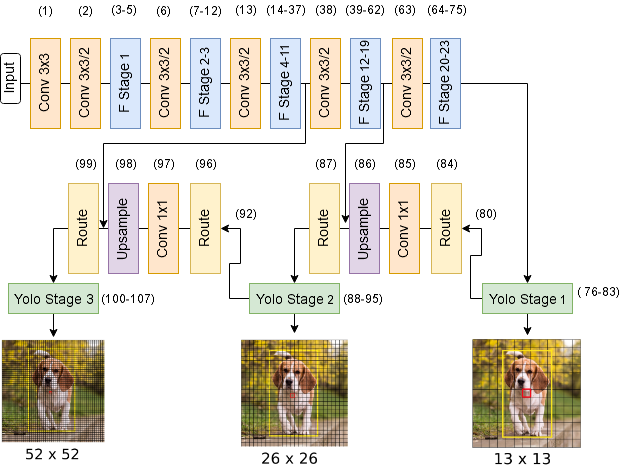
\includegraphics[width=0.85\textwidth]{Figures/CompleteYolov3Diagram.png}
	\caption[Caption for figure in TOC.]{Diagram of Yolov3 network}
	\label{fig:Yolov3_complete}
\end{figure}

The first part of the network is composed of a series of convolutional layers
terminated by F stages. Convolutional layers with stride 2 reduce the FMs by a
factor of four along the way. In this network implementation, the convolutions
use zero padding around the input FMs, so the size is maintained in the output
FMs. This part of the network is responsible for the feature detection in the
input image.

The second part of the netwok begins with a Yolo stage after which there is a
route layer that concatenates the output of the layers indicated in
Fig.~\ref{fig:Yolov3_complete}. This output is then compacted in terms of depth
by a $1\times 1$ convolution and upsampled by a factor of 2 in each FM
dimension, preparing the FMs for detections in a grid of $26\times26$ cells and
consequently detecting smaller objects in the image. These FMs are then
concatenated with the set of FMs of the same size from the detection part of the
network. The combination of the outputs of these two layers contribute with more
meaningfulness using the information from the upsampled layer and the
finer-grained information from the earlier feature maps~\cite{yolov3}.

After condensing the depth of the layer output to 255 FMs (again with a
convolutional layer with $1\times 1$ kernels), a second Yolo stage is used for
object detection at the new scale. The process is repeated one more time for the
third detection at the last yolo stage for a $52\times52$ grid.


\subsection{Tiny-YOLOv3}
\label{sec:tiny-yolov3}
For constrained environments, a small version of YOLOv3 is available. The layer
composition of the network is presented in
Tab.~\ref{tab:yolov3_tiny_num_layers}.

\begin{figure}[!htb]
	\begin{minipage}[b]{0.5\linewidth}
		\centering
		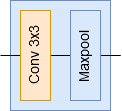
\includegraphics[width=0.35\textwidth]{Figures/TinyStage.png}
		\caption{Tiny-Yolov3 stage composition}
		\label{fig:Tiny_Stage}
	\end{minipage}%
	\begin{minipage}[b]{0.5\linewidth}
		\centering
		\begin{tabular}{lc}
			\toprule
			Layer Type           & Number of Layers  \\
			\midrule
			Convolutional       & 13    \\
			Maxpool  			& 6     \\
			Route 			    & 2     \\
			Yolo  				& 2     \\
			Upsample 		    & 1     \\
			Total 				& 24 \\
			\bottomrule
			
		\end{tabular}
		\caption[Table caption shown in TOC.]{Tiny-Yolov3 layer type composition.}
		\label{tab:yolov3_tiny_num_layers}
	\end{minipage}
\end{figure}

The first part of the network is composed of repeated Tiny-Yolov3 stages
presented in Fig.~\ref{fig:Tiny_Stage}. Each stage is composed of a
convolutional layer with $3\times3$ followed by a maxpooling layer.

This network follows the same sequence of layers present in Yolov3. The main
differences are in the number of layers and in the number of detections
performed. The Tiny-Yolov3 network performs object detection at only 2 grid
resolutions: $13\times13$ and $26\times26$.

\section*{Final Remark}
State-of-the-art CNN models are widely used for object detection
applications. These networks rely on convolution to extract features from the
images in order to be able to perform object detection. In order to achieve
higher performance metrics, CNNs grow in complexity. The Yolov3~\cite{yolov3}
network obtains comparable mAP for the COCO dataset~\cite{coco:Microsoft} to
other networks, at a fraction of the inference time.



